% The Gaussian e^{-\pi x^2} against the scaled Gaussian e^{-\pi x^2/4}.
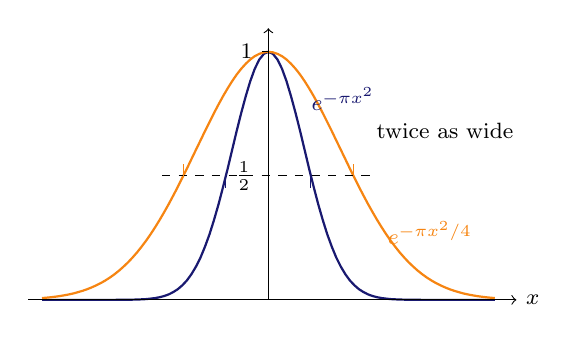
\begin{tikzpicture}[every node/.style={font=\footnotesize}]
\draw[MidnightBlue,thick] (-2.875,0.000)--(-2.817,0.000)--(-2.760,0.000)--(-2.702,0.000)--(-2.645,0.000)--(-2.587,0.000)--(-2.530,0.000)--(-2.472,0.000)--(-2.415,0.000)--(-2.357,0.000)--(-2.300,0.000)--(-2.243,0.000)--(-2.185,0.000)--(-2.127,0.000)--(-2.070,0.000)--(-2.012,0.000)--(-1.955,0.000)--(-1.897,0.001)--(-1.840,0.001)--(-1.782,0.002)--(-1.725,0.003)--(-1.667,0.004)--(-1.610,0.007)--(-1.552,0.010)--(-1.495,0.016)--(-1.438,0.023)--(-1.380,0.034)--(-1.323,0.049)--(-1.265,0.070)--(-1.208,0.099)--(-1.150,0.136)--(-1.093,0.185)--(-1.035,0.247)--(-0.978,0.325)--(-0.920,0.422)--(-0.862,0.538)--(-0.805,0.676)--(-0.747,0.835)--(-0.690,1.017)--(-0.632,1.218)--(-0.575,1.436)--(-0.517,1.667)--(-0.460,1.906)--(-0.403,2.144)--(-0.345,2.374)--(-0.287,2.588)--(-0.230,2.778)--(-0.173,2.935)--(-0.115,3.053)--(-0.057,3.125)--(0.000,3.150)--(0.057,3.125)--(0.115,3.053)--(0.173,2.935)--(0.230,2.778)--(0.287,2.588)--(0.345,2.374)--(0.403,2.144)--(0.460,1.906)--(0.517,1.667)--(0.575,1.436)--(0.632,1.218)--(0.690,1.017)--(0.747,0.835)--(0.805,0.676)--(0.862,0.538)--(0.920,0.422)--(0.978,0.325)--(1.035,0.247)--(1.093,0.185)--(1.150,0.136)--(1.208,0.099)--(1.265,0.070)--(1.323,0.049)--(1.380,0.034)--(1.438,0.023)--(1.495,0.016)--(1.552,0.010)--(1.610,0.007)--(1.667,0.004)--(1.725,0.003)--(1.782,0.002)--(1.840,0.001)--(1.897,0.001)--(1.955,0.000)--(2.012,0.000)--(2.070,0.000)--(2.127,0.000)--(2.185,0.000)--(2.243,0.000)--(2.300,0.000)--(2.357,0.000)--(2.415,0.000)--(2.472,0.000)--(2.530,0.000)--(2.587,0.000)--(2.645,0.000)--(2.702,0.000)--(2.760,0.000)--(2.817,0.000)--(2.875,0.000);
\draw[BurntOrange,thick] (-2.875,0.023)--(-2.817,0.028)--(-2.760,0.034)--(-2.702,0.041)--(-2.645,0.049)--(-2.587,0.059)--(-2.530,0.070)--(-2.472,0.083)--(-2.415,0.099)--(-2.357,0.116)--(-2.300,0.136)--(-2.243,0.159)--(-2.185,0.185)--(-2.127,0.214)--(-2.070,0.247)--(-2.012,0.284)--(-1.955,0.325)--(-1.897,0.371)--(-1.840,0.422)--(-1.782,0.477)--(-1.725,0.538)--(-1.667,0.604)--(-1.610,0.676)--(-1.552,0.753)--(-1.495,0.835)--(-1.438,0.923)--(-1.380,1.017)--(-1.323,1.115)--(-1.265,1.218)--(-1.208,1.325)--(-1.150,1.436)--(-1.093,1.551)--(-1.035,1.667)--(-0.978,1.786)--(-0.920,1.906)--(-0.862,2.025)--(-0.805,2.144)--(-0.747,2.260)--(-0.690,2.374)--(-0.632,2.484)--(-0.575,2.588)--(-0.517,2.687)--(-0.460,2.778)--(-0.403,2.861)--(-0.345,2.935)--(-0.287,2.999)--(-0.230,3.053)--(-0.173,3.095)--(-0.115,3.125)--(-0.057,3.144)--(0.000,3.150)--(0.057,3.144)--(0.115,3.125)--(0.173,3.095)--(0.230,3.053)--(0.287,2.999)--(0.345,2.935)--(0.403,2.861)--(0.460,2.778)--(0.517,2.687)--(0.575,2.588)--(0.632,2.484)--(0.690,2.374)--(0.747,2.260)--(0.805,2.144)--(0.862,2.025)--(0.920,1.906)--(0.978,1.786)--(1.035,1.667)--(1.093,1.551)--(1.150,1.436)--(1.208,1.325)--(1.265,1.218)--(1.323,1.115)--(1.380,1.017)--(1.438,0.923)--(1.495,0.835)--(1.552,0.753)--(1.610,0.676)--(1.667,0.604)--(1.725,0.538)--(1.782,0.477)--(1.840,0.422)--(1.897,0.371)--(1.955,0.325)--(2.012,0.284)--(2.070,0.247)--(2.127,0.214)--(2.185,0.185)--(2.243,0.159)--(2.300,0.136)--(2.357,0.116)--(2.415,0.099)--(2.472,0.083)--(2.530,0.070)--(2.587,0.059)--(2.645,0.049)--(2.702,0.041)--(2.760,0.034)--(2.817,0.028)--(2.875,0.023);
\draw[black,dashed] (-1.35,1.575)--(1.35,1.575);
\draw[MidnightBlue] (0.540,1.575)--(0.540,1.42);
\draw[MidnightBlue] (-0.540,1.575)--(-0.540,1.42);
\draw[BurntOrange] (1.080,1.575)--(1.080,1.73);
\draw[BurntOrange] (-1.080,1.575)--(-1.080,1.73);
\draw[->] (-3.05,0)--(3.15,0) node[right] {$x$};
\draw[->] (0,0)--(0,3.45);
\draw (0,3.15)--(-0.08,3.15) node[left] {$1$};
\draw (0,1.575)--(-0.08,1.575) node[left] {$\frac12$};
\node[MidnightBlue] at (0.95,2.55) {$e^{-\pi x^2}$};
\node[BurntOrange] at (2.05,0.85) {$e^{-\pi x^2/4}$};
\node[anchor=west] at (1.25,2.15) {twice as wide};
\end{tikzpicture}
